\documentclass[aspectratio=169,11pt]{beamer}
\usepackage[T1]{fontenc}
\usepackage[utf8]{inputenc}
\usepackage[english]{babel}
\usepackage{lmodern,amsmath,booktabs,tikz}
\definecolor{ink}{HTML}{172D43}
\definecolor{simple}{HTML}{2166AC}
\definecolor{pivot}{HTML}{D66014}
\setbeamercolor{normal text}{fg=ink,bg=white}
\setbeamercolor{frametitle}{fg=ink}
\setbeamercolor{structure}{fg=simple}
\setbeamercolor{block title}{fg=ink,bg=simple!12}
\setbeamercolor{block body}{fg=ink,bg=simple!4}
\setbeamerfont{frametitle}{size=\Large,series=\bfseries}
\setbeamertemplate{navigation symbols}{}
\setbeamertemplate{bibliography item}{\insertbiblabel}
\setbeamercolor{bibliography entry author}{fg=ink}
\setbeamercolor{bibliography entry title}{fg=ink}
\setbeamercolor{bibliography entry location}{fg=ink}
\setbeamercolor{bibliography entry note}{fg=ink}
\setbeamertemplate{footline}{}
\setbeamersize{text margin left=7mm,text margin right=7mm}
\graphicspath{{figures/}}
\newcommand{\source}[1]{\par\vspace{1mm}{\tiny\color{gray}#1}}
\begin{document}
% Generated by scripts/plot_corrected_fit.py; do not edit values by hand.
\newcommand{\correctedA}{0.7704\pm0.0004}
\newcommand{\correctedNu}{0.75005\pm0.00003}
\newcommand{\correctedB}{1.8\pm0.2}
\newcommand{\correctedC}{-6\pm2}
\newcommand{\correctedChi}{17.42}
\newcommand{\correctedReducedChi}{1.02}
\newcommand{\correctedDof}{17}

\begin{frame}[plain]
\begin{tikzpicture}[remember picture,overlay]
% A quiet side panel frames the title.
\fill[simple!4] ([xshift=-39mm]current page.north east) rectangle (current page.south east);

\node[anchor=south,inner sep=0pt] at ([xshift=-19.5mm,yshift=9mm]current page.south east) {
\includegraphics[width=29mm]{logo.png}};
\node[anchor=north east,align=right,inner sep=0pt,text=ink!75,font=\small] at ([xshift=-8mm,yshift=-9mm]current page.north east) {Bachelor's Degree\\in Physics};
\node[anchor=west,inner sep=0pt,fill=white,minimum height=13mm] at ([xshift=9mm,yshift=10mm]current page.west) {{\LARGE\bfseries Two-dimensional self-avoiding walks}};
\node[anchor=west,inner sep=0pt,font=\large,text=ink!85] at ([xshift=9mm,yshift=-2mm]current page.west) {Direct rejection and the Pivot algorithm};
\draw[pivot,line width=1.5pt] ([xshift=9mm,yshift=-12mm]current page.west) -- ++(14mm,0);
% Separate baselines keep both labels and both names precisely aligned.
\node[anchor=base west,inner sep=0pt,font=\small] at ([xshift=9mm,yshift=26mm]current page.south west) {Candidate};
\node[anchor=base west,inner sep=0pt,font=\small] at ([xshift=65mm,yshift=26mm]current page.south west) {Supervisor};
\node[anchor=base west,inner sep=0pt,font=\large\bfseries] at ([xshift=9mm,yshift=18mm]current page.south west) {Jacopo Martellotto};
\node[anchor=base west,inner sep=0pt,font=\large\bfseries] at ([xshift=65mm,yshift=18mm]current page.south west) {Prof.\ Claudio Bonati};
\end{tikzpicture}
\end{frame}
\begin{frame}{Self-avoidance and polymer scaling}
\begin{tikzpicture}[remember picture,overlay]
\begin{scope}[shift={(current page.north west)},x=1mm,y=-1mm]
\node[anchor=north west,text width=145mm,inner sep=0pt,
font=\fontsize{8.5}{9.5}\selectfont] at (7,11.5)
{A \textbf{self-avoiding walk} never revisits a lattice site. It models excluded volume in a good solvent.\par
$R_e$ is one walk's end-to-end distance; $R$ is a trial chain size, whose Flory optimum satisfies $R_*\sim\sqrt{\langle R_e^2\rangle}$.\par
$d$ is the spatial dimension and $v>0$ measures excluded-volume repulsion.};

% A single large sketch introduces the measured extension.
\fill[simple!3,rounded corners=1.2mm] (7,24) rectangle (51,67);
\node[anchor=north west,inner sep=0pt,text=simple,
font=\fontsize{9.5}{10}\selectfont\bfseries] at (11,27) {A self-avoiding chain};
\node[anchor=north west,inner sep=0pt] at (12,34) {
\begin{tikzpicture}[x=1cm,y=1cm,scale=.52,>=stealth]
\draw[step=1,ink!13,thin] (-.3,-.3) grid (5.3,4.3);
\draw[simple,line width=1.5pt] (0,0)--(1,0)--(1,1)--(0,1)--(0,2)--(1,2)--(2,2)--(2,1)--(3,1)--(3,2)--(4,2)--(4,3)--(3,3)--(2,3)--(2,4)--(3,4)--(4,4)--(5,4);
\foreach \x/\y in {0/0,1/0,1/1,0/1,0/2,1/2,2/2,2/1,3/1,3/2,4/2,4/3,3/3,2/3,2/4,3/4,4/4,5/4}{\fill[simple] (\x,\y) circle(.09);}
\draw[ink!70,dashed,->,line width=.85pt] (.1,.08)--(4.88,3.9);
\node[fill=white,inner sep=1pt,font=\fontsize{8}{8}\selectfont,text=ink] at (2.6,1.7) {$R_e$};
\fill[ink] (0,0) circle(.13);
\fill[pivot] (5,4) circle(.13);
\end{tikzpicture}};
\node[anchor=north west,inner sep=0pt,font=\fontsize{8.5}{9.3}\selectfont] at (10,68.5)
{$N$ steps of length $a$};
\node[anchor=north west,inner sep=0pt,font=\fontsize{9}{10}\selectfont] at (10,73)
{$R_e^2=|\mathbf r_N-\mathbf r_0|^2$};

% Two competing contributions, with only their leading dependence.
\fill[simple!5,rounded corners=1.2mm] (59,24) rectangle (102,48.7);
\fill[pivot!6,rounded corners=1.2mm] (109,24) rectangle (153,48.7);
\node[anchor=north west,inner sep=0pt,font=\fontsize{9.2}{10}\selectfont\bfseries,text=simple] at (62,26.5)
{Entropic elasticity};
\node[anchor=north west,inner sep=0pt,font=\fontsize{9.2}{10}\selectfont\bfseries,text=pivot] at (112,26.5)
{Excluded volume};
\node[font=\fontsize{12}{12.5}\selectfont,text=simple] at (80.5,36)
{$\displaystyle \frac{F_{\mathrm{el}}}{k_BT}\sim\frac{R^2}{Na^2}$};
\node[font=\fontsize{12}{12.5}\selectfont,text=pivot] at (131,36)
{$\displaystyle \frac{F_{\mathrm{int}}}{k_BT}\sim\frac{vN^2}{R^d}$};
\node[anchor=north west,inner sep=0pt,font=\fontsize{8}{8.8}\selectfont] at (62,43)
{Stretching reduces entropy.};
\node[anchor=north west,text width=38mm,inner sep=0pt,font=\fontsize{8}{8.8}\selectfont] at (112,42.5)
{Crowding reduces the number of allowed conformations.};

% A short mathematical chain leads directly to the result.
\node[anchor=north west,inner sep=0pt,font=\fontsize{9.5}{10}\selectfont\bfseries] at (60,50.5)
{Flory approximation};
\node[anchor=west,inner sep=0pt,font=\fontsize{11}{12}\selectfont] at (60,59.5)
{$\displaystyle \frac{F_{\rm F}(R)}{k_{\rm B}T}
\sim {\color{simple}\frac{R^2}{Na^2}}+
{\color{pivot}\frac{vN^2}{R^d}}$};
\node[anchor=west,inner sep=0pt,font=\fontsize{10}{11}\selectfont] at (60,66.8)
{$\displaystyle \text{Minimise in }R
\quad\Longrightarrow\quad R_*\sim aN^{\nu_F},\qquad \nu_F=\frac{3}{d+2}$};
\node[anchor=north west,text width=93mm,inner sep=0pt,text=ink!70,
font=\fontsize{7.8}{9}\selectfont] at (60,71.8)
{Gaussian elasticity, uniform density, leading pair repulsion.\par
Asymptotic scaling for $N\gg1$ with $v\sim a^d>0$.};

% The main result is the strongest visual element.
\fill[ink,rounded corners=1mm] (7,79.5) rectangle (153,85.5);
\node[anchor=west,inner sep=0pt,text=white,font=\fontsize{9.5}{10}\selectfont\bfseries] at (11,82.5)
{In two dimensions:};
\node[text=white,font=\fontsize{12}{12.5}\selectfont] at (94,82.5)
{$\displaystyle \nu_F=\tfrac34
\quad\Longrightarrow\quad \langle R_e^2\rangle\sim R_*^2\sim a^2N^{3/2}$};
\node[anchor=east,inner sep=0pt,text=white!80,font=\fontsize{8}{8.5}\selectfont] at (150,82.5)
{$a=1$};
\end{scope}
\end{tikzpicture}
\end{frame}

\begin{frame}{Simple sampling by direct rejection}
\begin{tikzpicture}[remember picture,overlay]
\begin{scope}[shift={(current page.north west)},x=1mm,y=-1mm]
\node[anchor=north west,text width=145mm,inner sep=0pt,text=ink!80,
font=\fontsize{9}{10}\selectfont] at (7,12)
{Grow independent lattice walks; reject the whole trial at the first repeated site.};

% Four generous panels make the sequence readable without a dense sidebar.
\fill[simple!3,rounded corners=1.2mm] (7,21.5) rectangle (77,46.5);
\fill[simple!3,rounded corners=1.2mm] (83,21.5) rectangle (153,46.5);
\fill[pivot!4,rounded corners=1.2mm] (7,50.5) rectangle (77,75.5);
\fill[simple!3,rounded corners=1.2mm] (83,50.5) rectangle (153,75.5);

\fill[simple] (12.5,26.5) circle (3.1);
\node[text=white,font=\fontsize{8.5}{9}\selectfont\bfseries] at (12.5,26.5) {1};
\node[anchor=west,inner sep=0pt,font=\fontsize{10}{10.5}\selectfont\bfseries] at (18,26.5) {Start};
\node[anchor=north west,inner sep=0pt] at (10,31.5) {
\begin{tikzpicture}[x=1cm,y=1cm,scale=.30]
\draw[step=1,ink!15,thin] (-.2,-.2) grid (4.2,4.2);
\fill[simple] (2,1) circle(.17);
\end{tikzpicture}};
\node[anchor=north west,text width=39mm,inner sep=0pt,
font=\fontsize{8.7}{10}\selectfont,align=left] at (32,32.5)
{Start at the origin.\par Mark it as visited.};

\fill[simple] (88.5,26.5) circle (3.1);
\node[text=white,font=\fontsize{8.5}{9}\selectfont\bfseries] at (88.5,26.5) {2};
\node[anchor=west,inner sep=0pt,font=\fontsize{10}{10.5}\selectfont\bfseries] at (94,26.5) {Propose a step};
\node[anchor=north west,inner sep=0pt] at (86,31.5) {
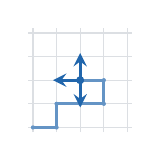
\begin{tikzpicture}[x=1cm,y=1cm,scale=.30,>=stealth]
\draw[step=1,ink!15,thin] (-.2,-.2) grid (4.2,4.2);
\draw[simple!70,line width=1.1pt] (0,0)--(1,0)--(1,1)--(2,1)--(3,1)--(3,2)--(2,2);
\foreach \x/\y in {0/0,1/0,1/1,2/1,3/1,3/2}{\fill[simple!70] (\x,\y) circle(.09);}
\fill[simple] (2,2) circle(.17);
\draw[->,simple,line width=1.1pt] (2,2)--(.85,2);
\draw[->,simple,line width=1.1pt] (2,2)--(2,3.15);
\draw[->,simple,line width=1.1pt] (2,2)--(2,.85);
\end{tikzpicture}};
\node[anchor=north west,text width=42mm,inner sep=0pt,
font=\fontsize{8}{9}\selectfont,align=left] at (108,32)
{No reversal: $1/3$ per direction.\par
A reversal fails the site check.};

\fill[pivot] (12.5,55.5) circle (3.1);
\node[text=white,font=\fontsize{8.5}{9}\selectfont\bfseries] at (12.5,55.5) {3};
\node[anchor=west,inner sep=0pt,font=\fontsize{10}{10.5}\selectfont\bfseries] at (18,55.5) {Check the site};
\node[anchor=north west,inner sep=0pt] at (10,60.5) {
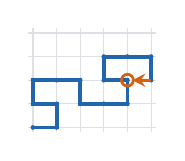
\begin{tikzpicture}[x=1cm,y=1cm,scale=.30,>=stealth]
\draw[step=1,ink!15,thin] (-.2,-.2) grid (5.2,4.2);
\draw[simple,line width=1.4pt] (0,0)--(1,0)--(1,1)--(0,1)--(0,2)--(1,2)--(2,2)--(2,1)--(3,1)--(4,1)--(4,2)--(3,2)--(3,3)--(4,3)--(5,3)--(5,2);
\foreach \x/\y in {0/0,1/0,1/1,0/1,0/2,1/2,2/2,2/1,3/1,4/1,4/2,3/2,3/3,4/3,5/3,5/2}{\fill[simple] (\x,\y) circle(.1);}
\draw[->,pivot,line width=1.1pt] (5,2)--(4.2,2);
\draw[pivot,line width=1pt] (4,2) circle(.25);
\end{tikzpicture}};
\node[anchor=north west,text width=40mm,inner sep=0pt,
font=\fontsize{8.3}{9.4}\selectfont,align=left] at (32,61)
{{\color{simple}\bfseries New site:} continue.\par\vspace{.7mm}
{\color{pivot}\bfseries Visited site:} reject and restart.};

\fill[simple] (88.5,55.5) circle (3.1);
\node[text=white,font=\fontsize{8.5}{9}\selectfont\bfseries] at (88.5,55.5) {4};
\node[anchor=west,inner sep=0pt,font=\fontsize{10}{10.5}\selectfont\bfseries] at (94,55.5) {Accept and measure};
\node[anchor=north west,inner sep=0pt] at (86,60.5) {
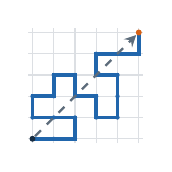
\begin{tikzpicture}[x=1cm,y=1cm,scale=.27,>=stealth]
\draw[step=1,ink!15,thin] (-.2,-.2) grid (5.2,5.2);
\draw[simple,line width=1.4pt] (0,0)--(1,0)--(2,0)--(2,1)--(1,1)--(0,1)--(0,2)--(1,2)--(1,3)--(2,3)--(2,2)--(3,2)--(3,1)--(4,1)--(4,2)--(4,3)--(3,3)--(3,4)--(4,4)--(5,4)--(5,5);
\foreach \x/\y in {0/0,1/0,2/0,2/1,1/1,0/1,0/2,1/2,1/3,2/3,2/2,3/2,3/1,4/1,4/2,4/3,3/3,3/4,4/4,5/4,5/5}{\fill[simple] (\x,\y) circle(.1);}
\draw[->,ink!70,dashed,line width=.85pt] (.12,.12)--(4.88,4.88);
\fill[ink] (0,0) circle(.14);
\fill[pivot] (5,5) circle(.14);
\end{tikzpicture}};
\node[anchor=north west,text width=39mm,inner sep=0pt,
font=\fontsize{8.7}{9.8}\selectfont,align=left] at (108,61)
{After $N$ valid steps,\par accept the walk.};
\node[anchor=west,inner sep=0pt,font=\fontsize{9}{10}\selectfont] at (108,71.5)
{$R_e^2=|\mathbf r_N-\mathbf r_0|^2$};

\fill[simple!7,rounded corners=1mm] (7,80) rectangle (153,85);
\node[anchor=west,inner sep=0pt,font=\fontsize{8.7}{9.5}\selectfont\bfseries,text=simple] at (11,82.5)
{Observables and scaling};
\node[font=\fontsize{10}{10.5}\selectfont] at (104,82.5)
{$\langle R_e^2\rangle\propto N^{2\nu}\qquad P_{\rm success}\qquad \nu\ \text{(fit)}$};
\end{scope}
\end{tikzpicture}
\end{frame}
\begin{frame}{The Pivot algorithm: global shape updates}
\begin{tikzpicture}[remember picture,overlay]
\begin{scope}[shift={(current page.north west)},x=1mm,y=-1mm]
\node[anchor=north west,text width=145mm,inner sep=0pt,text=ink!80,
font=\fontsize{9}{10}\selectfont] at (7,12)
{Start from a straight SAW. A rigid lattice symmetry reshapes the tail of the current walk.\par
Each move preserves all $N$ lattice bonds. Successive configurations remain correlated.};

% The four numbered operations form one update cycle, repeated in both phases.
\node[anchor=west,inner sep=0pt,text=pivot,
font=\fontsize{8.2}{9}\selectfont\bfseries] at (7,22)
{One Pivot attempt};
\fill[pivot!3,rounded corners=1.2mm] (7,25) rectangle (41,59);
\fill[pivot!3,rounded corners=1.2mm] (44,25) rectangle (78,59);
\fill[pivot!3,rounded corners=1.2mm] (81,25) rectangle (115,59);
\fill[simple!3,rounded corners=1.2mm] (118,25) rectangle (153,59);
\draw[->,>=stealth,ink!40,line width=.6pt] (41.2,41.5) -- (43.8,41.5);
\draw[->,>=stealth,ink!40,line width=.6pt] (78.2,41.5) -- (80.8,41.5);
\draw[->,>=stealth,ink!40,line width=.6pt] (115.2,41.5) -- (117.8,41.5);
\draw[->,>=stealth,ink!55,line width=.65pt,rounded corners=.8mm]
(135.5,59.5) -- (135.5,61.5) -- (24,61.5) -- (24,59.5);
\node[fill=white,inner xsep=2mm,inner ysep=.3mm,text=ink!80,
font=\fontsize{7.8}{8.8}\selectfont] at (79.75,61.5)
{Repeat from the current walk};
\fill[pivot!7,rounded corners=1mm] (7,63) rectangle (153,67);
\node[anchor=west,inner sep=0pt,font=\fontsize{8.1}{9}\selectfont] at (10,65)
{Seven equally likely moves: rotations by $90^\circ$, $180^\circ$, $270^\circ$ and reflections in axes or diagonals.};
\fill[ink!3,rounded corners=1.2mm] (7,69) rectangle (77,87);
\fill[pivot!4,rounded corners=1.2mm] (83,69) rectangle (153,87);
\draw[->,>=stealth,ink!45,line width=.65pt] (77.5,77.5) -- (82.5,77.5);

% 1. The same prefix and pivot are used throughout the geometric example.
\fill[pivot] (11.5,30) circle (3.1);
\node[text=white,font=\fontsize{8.5}{9}\selectfont\bfseries] at (11.5,30) {1};
\node[anchor=west,inner sep=0pt,font=\fontsize{8.7}{9.5}\selectfont\bfseries] at (17,30)
{Choose a pivot};
\node[anchor=center,inner sep=0pt] at (24,41.5) {
\begin{tikzpicture}[x=1cm,y=1cm,scale=.30]
\draw[step=1,ink!13,thin] (-.3,-.3) grid (4.3,4.3);
\draw[simple,line width=1.5pt] (0,0)--(1,0)--(1,1)--(2,1)--(2,2);
\draw[pivot,line width=1.5pt] (2,2)--(3,2)--(3,3)--(4,3)--(4,4);
\foreach \x/\y in {0/0,1/0,1/1,2/1}{\fill[simple] (\x,\y) circle(.1);}
\foreach \x/\y in {3/2,3/3,4/3,4/4}{\fill[pivot] (\x,\y) circle(.1);}
\fill[ink] (2,2) circle(.13);
\draw[ink,line width=.8pt] (2,2) circle(.24);
\node[fill=pivot!3,inner sep=.5pt,font=\fontsize{7.8}{8}\selectfont] at (1.6,2.5) {$k$};
\end{tikzpicture}};
\node[anchor=north west,text width=28mm,inner sep=0pt,
font=\fontsize{7.8}{8.8}\selectfont,align=left] at (10,50.5)
{Choose $k$ at random.\par
{\color{simple}Prefix} and {\color{pivot}tail}.};

% 2. A clockwise rotation preserves the tail geometry and all lattice bonds.
\fill[pivot] (48.5,30) circle (3.1);
\node[text=white,font=\fontsize{8.5}{9}\selectfont\bfseries] at (48.5,30) {2};
\node[anchor=west,inner sep=0pt,font=\fontsize{8.7}{9.5}\selectfont\bfseries] at (54,30)
{Transform tail};
\node[anchor=center,inner sep=0pt] at (61,41.5) {
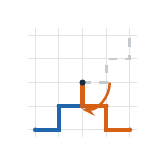
\begin{tikzpicture}[x=1cm,y=1cm,scale=.30,>=stealth]
\draw[step=1,ink!13,thin] (-.3,-.3) grid (4.3,4.3);
\draw[ink!25,dashed,line width=1pt] (2,2)--(3,2)--(3,3)--(4,3)--(4,4);
\draw[simple,line width=1.5pt] (0,0)--(1,0)--(1,1)--(2,1)--(2,2);
\draw[pivot,line width=1.5pt] (2,2)--(2,1)--(3,1)--(3,0)--(4,0);
\foreach \x/\y in {0/0,1/0,1/1,2/1}{\fill[simple] (\x,\y) circle(.1);}
\foreach \x/\y in {2/1,3/1,3/0,4/0}{\fill[pivot] (\x,\y) circle(.1);}
\fill[ink] (2,2) circle(.13);
\draw[->,pivot,line width=.9pt] (3.15,2) arc (0:-90:1.15);
\end{tikzpicture}};
\node[anchor=north west,text width=28mm,inner sep=0pt,
font=\fontsize{7.8}{8.8}\selectfont,align=left] at (47,50.5)
{Fix the {\color{simple}prefix}.\par Rotate or reflect.};

% 3. The proposed tail collides with the fixed prefix.
\fill[pivot] (85.5,30) circle (3.1);
\node[text=white,font=\fontsize{8.5}{9}\selectfont\bfseries] at (85.5,30) {3};
\node[anchor=west,inner sep=0pt,font=\fontsize{8.7}{9.5}\selectfont\bfseries] at (91,30)
{Check overlap};
\node[anchor=center,inner sep=0pt] at (98,41.5) {
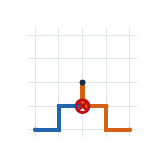
\begin{tikzpicture}[x=1cm,y=1cm,scale=.30]
\draw[step=1,ink!13,thin] (-.3,-.3) grid (4.3,4.3);
\draw[simple,line width=1.5pt] (0,0)--(1,0)--(1,1)--(2,1)--(2,2);
\draw[pivot,line width=1.5pt] (2,2)--(2,1)--(3,1)--(3,0)--(4,0);
\foreach \x/\y in {0/0,1/0,1/1}{\fill[simple] (\x,\y) circle(.1);}
\foreach \x/\y in {3/1,3/0,4/0}{\fill[pivot] (\x,\y) circle(.1);}
\fill[ink] (2,2) circle(.13);
\draw[red!75!ink,line width=1pt] (2,1) circle(.27);
\draw[red!75!ink,line width=.85pt] (1.84,.84)--(2.16,1.16) (1.84,1.16)--(2.16,.84);
\end{tikzpicture}};
\node[anchor=north west,text width=28mm,inner sep=0pt,
font=\fontsize{7.8}{8.8}\selectfont,align=left] at (84,50.5)
{Check the new tail\par against the prefix.};

% 4. This rejected proposal leaves the original walk unchanged.
\fill[pivot] (122.5,30) circle (3.1);
\node[text=white,font=\fontsize{8.5}{9}\selectfont\bfseries] at (122.5,30) {4};
\node[anchor=west,inner sep=0pt,font=\fontsize{8.7}{9.5}\selectfont\bfseries] at (128,30)
{Accept or reject};
\node[anchor=center,inner sep=0pt] at (135.5,41.5) {
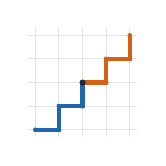
\begin{tikzpicture}[x=1cm,y=1cm,scale=.30]
\draw[step=1,ink!13,thin] (-.3,-.3) grid (4.3,4.3);
\draw[simple,line width=1.5pt] (0,0)--(1,0)--(1,1)--(2,1)--(2,2);
\draw[pivot,line width=1.5pt] (2,2)--(3,2)--(3,3)--(4,3)--(4,4);
\foreach \x/\y in {0/0,1/0,1/1,2/1}{\fill[simple] (\x,\y) circle(.1);}
\foreach \x/\y in {3/2,3/3,4/3,4/4}{\fill[pivot] (\x,\y) circle(.1);}
\fill[ink] (2,2) circle(.13);
\end{tikzpicture}};
\node[anchor=north west,text width=29mm,inner sep=0pt,
font=\fontsize{7.8}{8.8}\selectfont,align=left] at (121,50.5)
{{\color{simple}\bfseries Valid:} accept.\par
{\color{pivot}\bfseries Collision:} reject.};

% Thermalisation is a simulation phase, not a fifth operation in the cycle.
% Schematic straight and coiled walks have the same eight bonds.
\node[anchor=west,inner sep=0pt,text=ink!80,
font=\fontsize{9.3}{10}\selectfont\bfseries] at (30,73)
{Thermalisation};
\node[anchor=center,inner sep=0pt] at (19.5,78.5) {
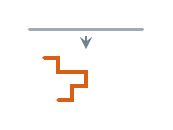
\begin{tikzpicture}[x=1cm,y=1cm,scale=.18,>=stealth]
\draw[ink!40,line width=1.2pt] (0,5)--(8,5);
\foreach \x in {0,...,8}{\fill[ink!40] (\x,5) circle(.1);}
\draw[->,ink!60,line width=.9pt] (4,4.5)--(4,3.6);
\draw[pivot,line width=1.5pt] (2,0)--(3,0)--(3,1)--(4,1)--(4,2)--(3,2)--(2,2)--(2,3)--(1,3);
\foreach \x/\y in {2/0,3/0,3/1,4/1,4/2,3/2,2/2,2/3,1/3}{\fill[pivot] (\x,\y) circle(.1);}
\end{tikzpicture}};
\node[anchor=north west,text width=43mm,inner sep=0pt,
font=\fontsize{8}{8.8}\selectfont,align=left] at (30,76.5)
{Repeat steps 1--4.\par
Discard initial attempts\par to reduce the starting bias.};

% Production repeats the same cycle with measurements enabled.
% Uniform measurement times include repetitions after rejected moves.
\node[anchor=west,inner sep=0pt,text=pivot,
font=\fontsize{9.3}{10}\selectfont\bfseries] at (108,73)
{Production};
\node[anchor=center,inner sep=0pt] at (96,79.5) {
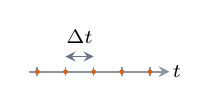
\begin{tikzpicture}[x=1cm,y=1cm,scale=.55,>=stealth]
\draw[->,ink!50,line width=.7pt] (0,0)--(3.25,0);
\foreach \x in {.2,.85,1.5,2.15,2.8}{
  \draw[ink!50,line width=.6pt] (\x,-.10)--(\x,.10);
  \fill[pivot] (\x,0) circle(.055);
}
\draw[<->,ink!65,line width=.6pt] (.85,.35)--(1.5,.35);
\node[anchor=south,inner sep=1pt,font=\fontsize{7}{7.5}\selectfont] at (1.175,.57) {$\Delta t$};
\node[anchor=west,inner sep=1pt,font=\fontsize{7}{7.5}\selectfont] at (3.25,0) {$t$};
\end{tikzpicture}};
\node[anchor=north west,text width=41mm,inner sep=0pt,
font=\fontsize{8}{8.8}\selectfont,align=left] at (108,76.5)
{Continue steps 1--4.\par
Record $R_e^2$ every $\Delta t$ attempts.\par
Include rejected moves.};
\end{scope}
\end{tikzpicture}
\end{frame}
\begin{frame}{Chain extension and sampling success}
\begin{tikzpicture}[remember picture,overlay]
\begin{scope}[shift={(current page.north west)},x=1mm,y=-1mm]
% Use the requested original figures without cropping or changing their data.
\node[anchor=north west,inner sep=0pt] at (7,12)
{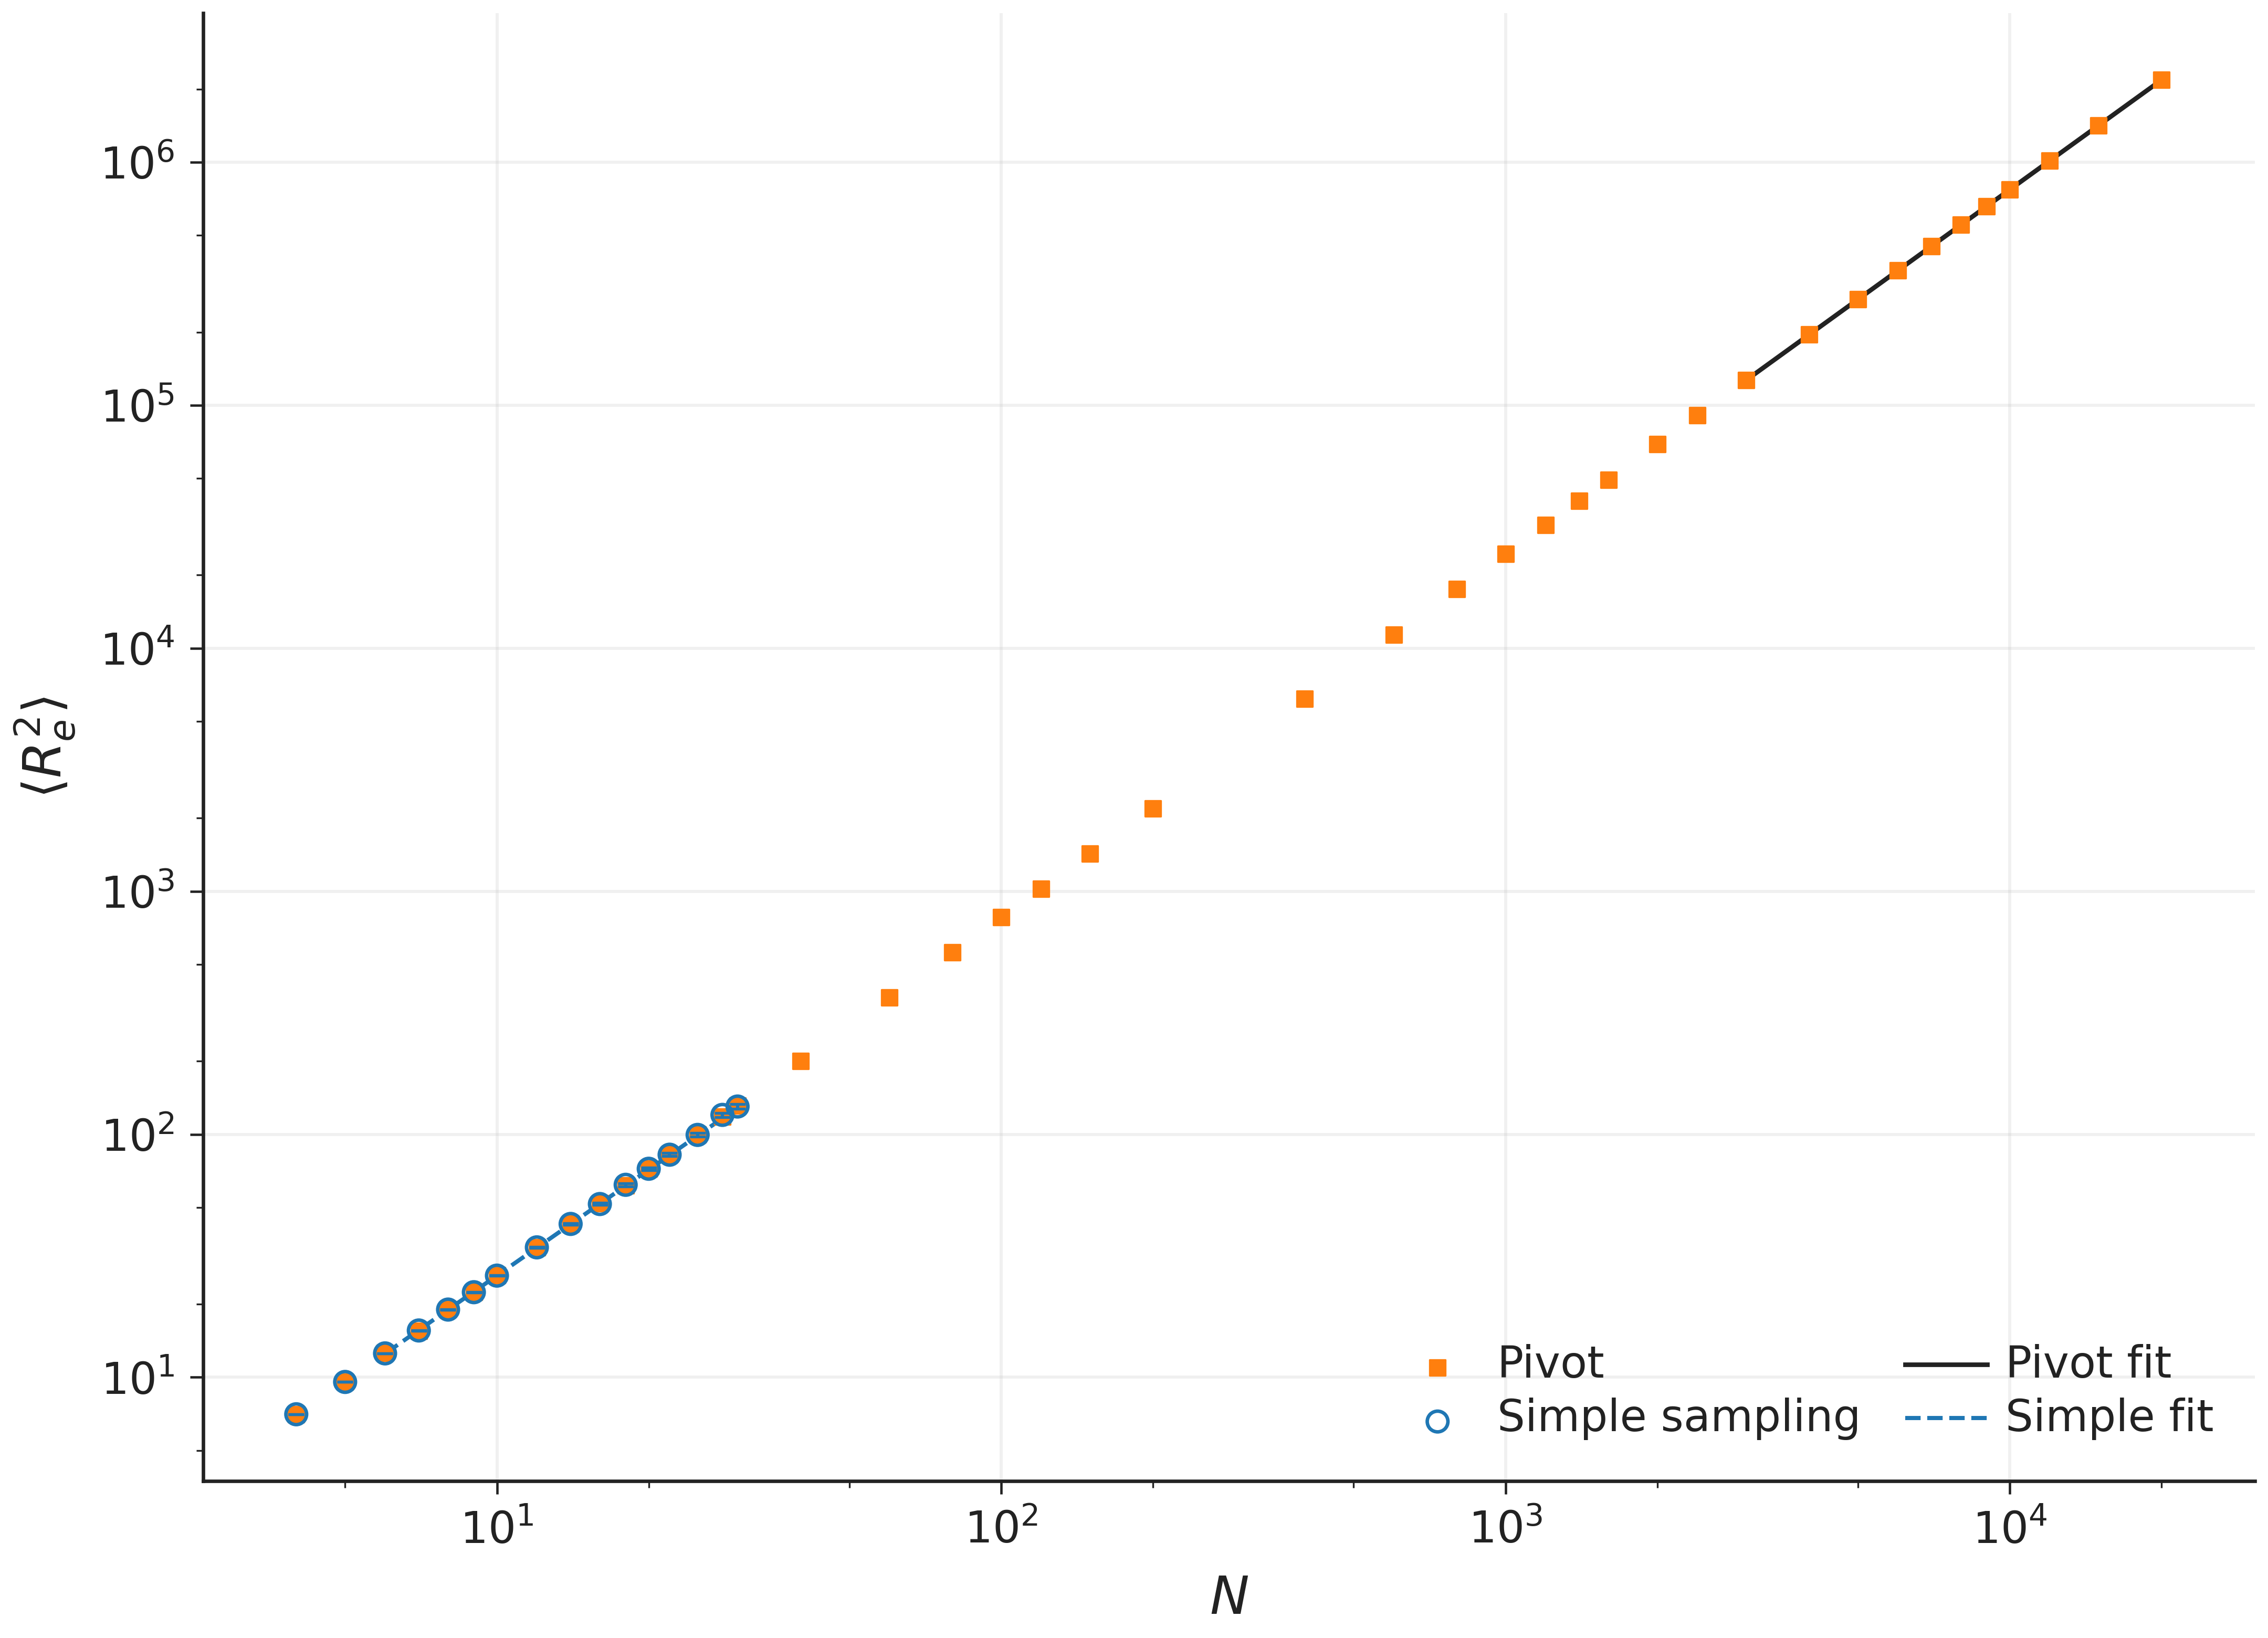
\includegraphics[width=71mm]{01_estensione.png}};
\node[anchor=north west,inner sep=0pt] at (82,12)
{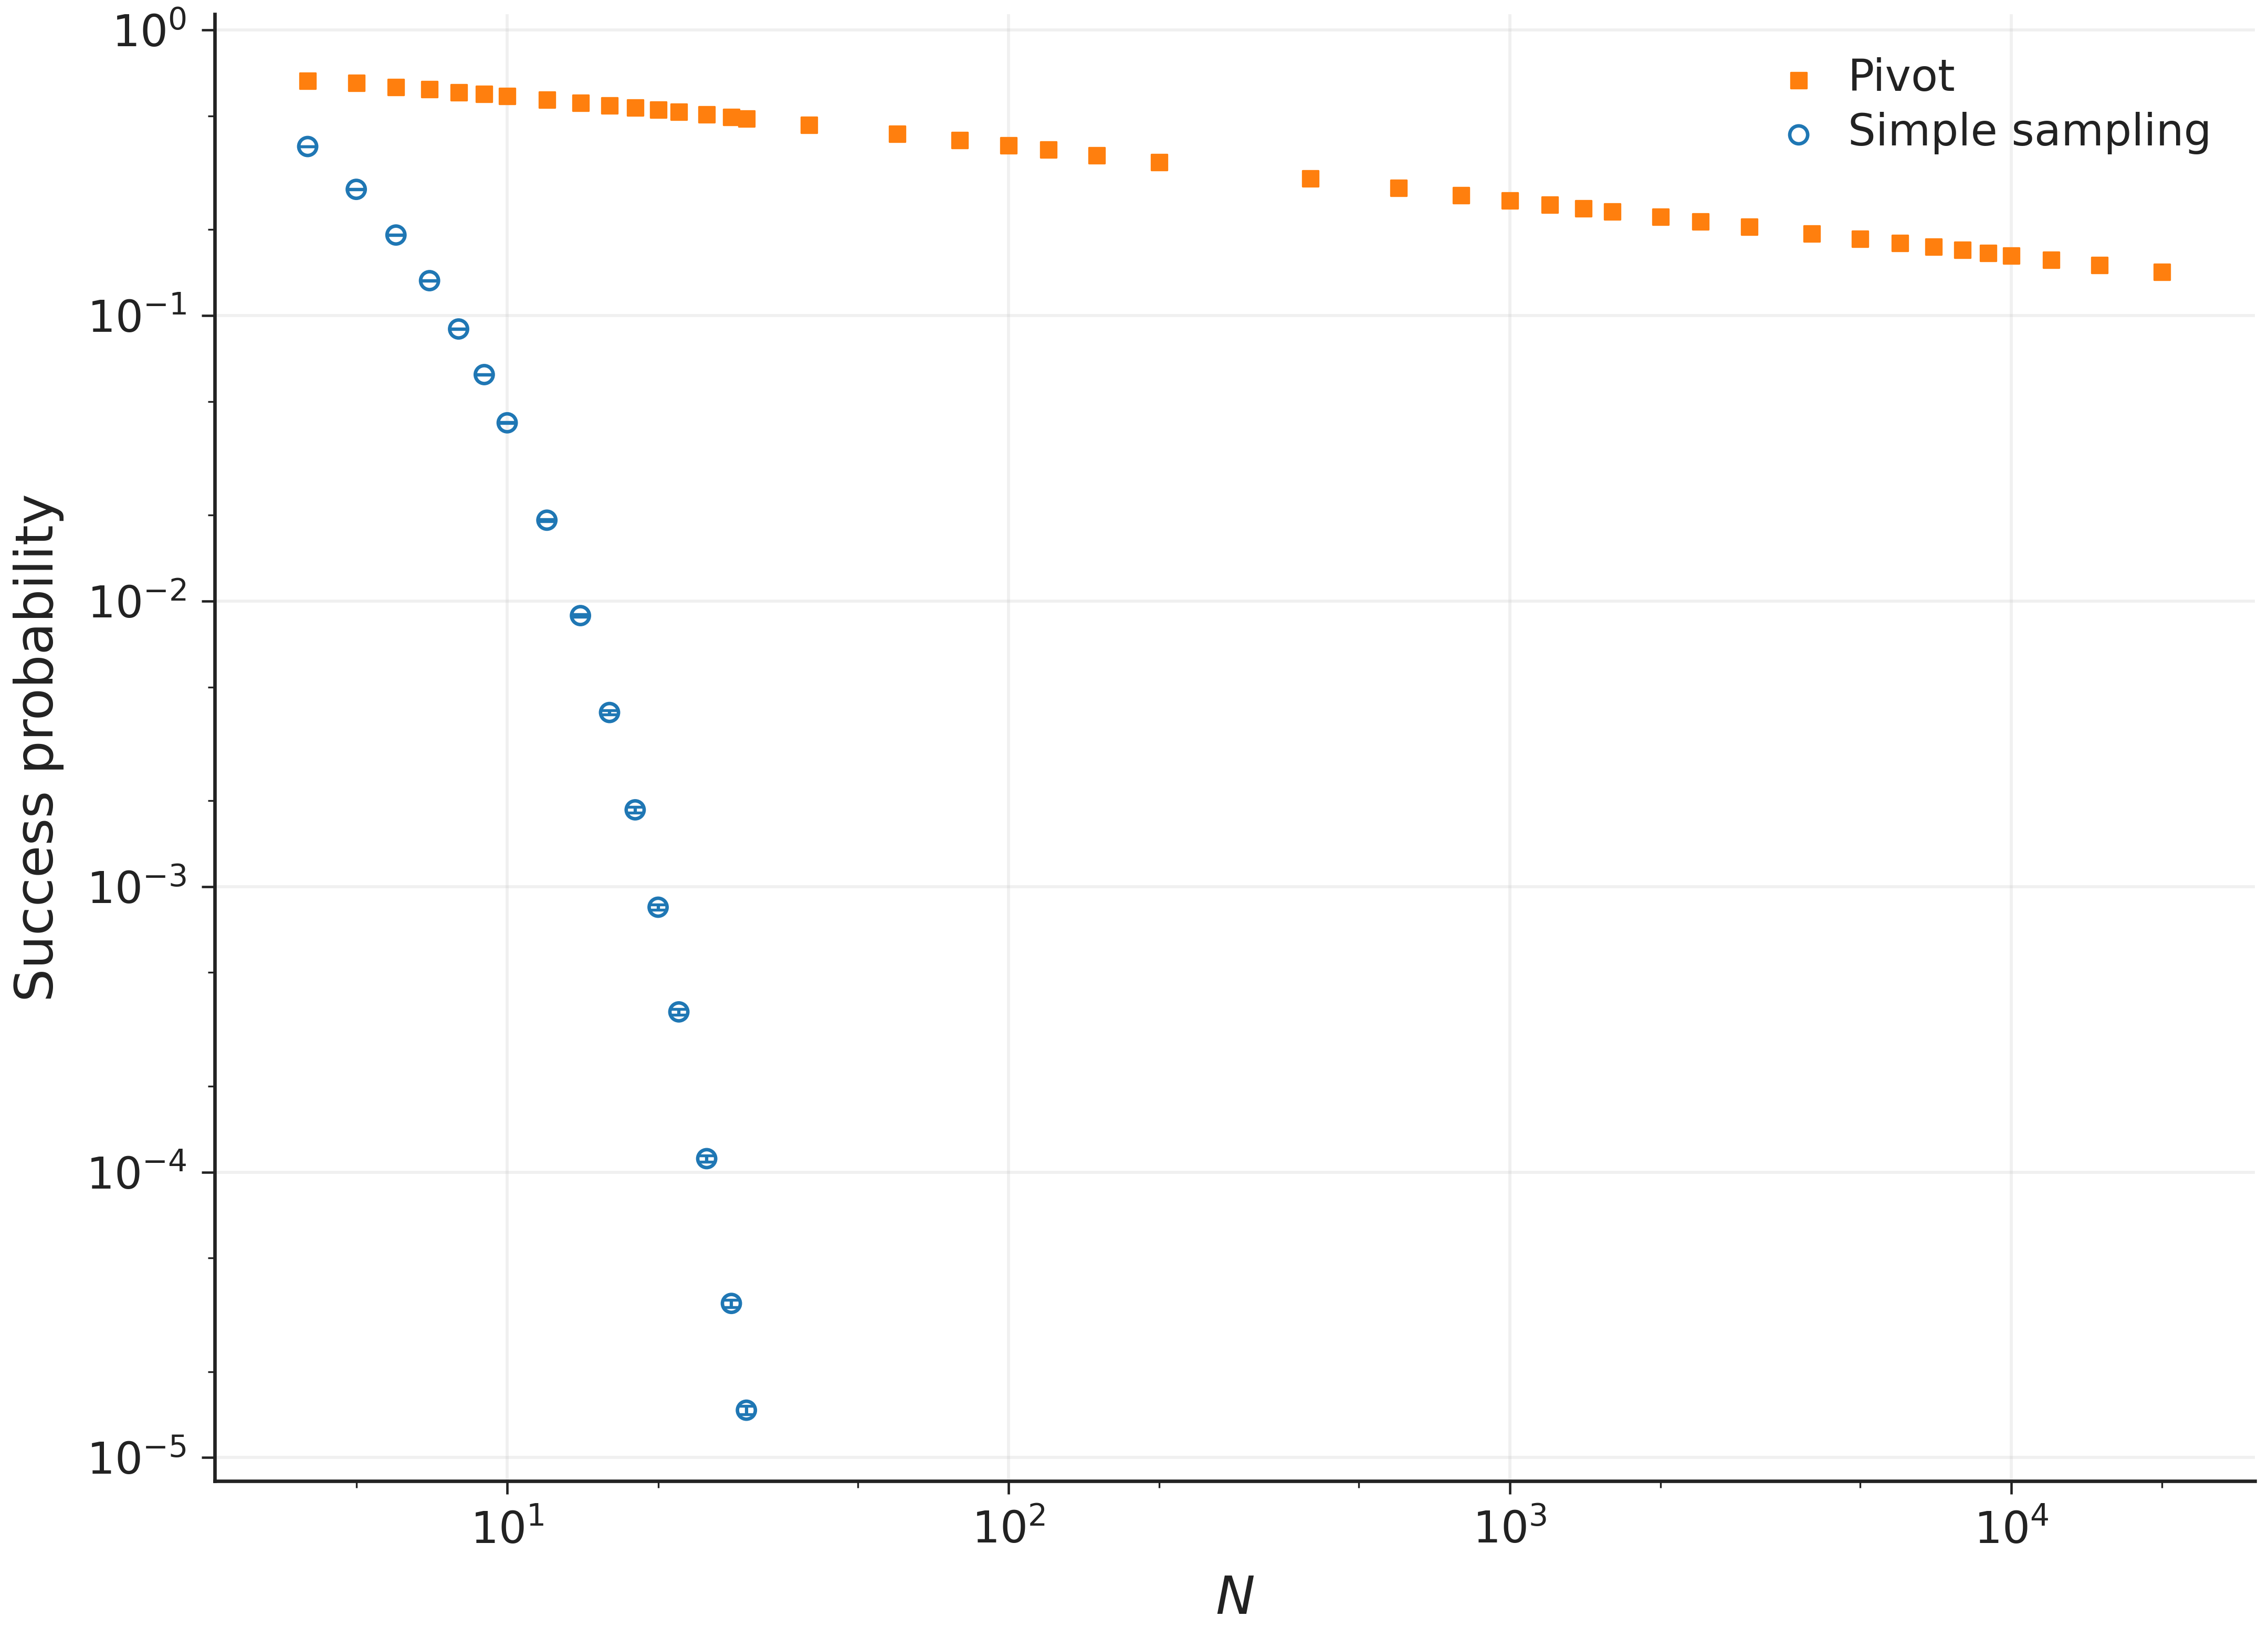
\includegraphics[width=71mm]{02_success_probability.png}};

\draw[ink!15,line width=.4pt] (7,66) -- (153,66);
\node[anchor=north west,inner sep=0pt,text=simple,
font=\fontsize{10}{11}\selectfont\bfseries] at (10,68.5)
{Simple sampling};
\node[anchor=north west,inner sep=0pt,text=pivot,
font=\fontsize{10}{11}\selectfont\bfseries] at (85,68.5)
{Pivot};
% Final pure-power-law estimates from the completed reproducible run.
\node[anchor=north west,inner sep=0pt,
font=\fontsize{12}{13}\selectfont] at (10,74)
% One-sigma covariance errors from curve_fit with absolute_sigma=True.
{$\nu=0.724\pm0.002$};
\node[anchor=north west,inner sep=0pt,
font=\fontsize{12}{13}\selectfont] at (85,74)
{$\nu=0.74996\pm0.00003$};

\node[anchor=west,inner sep=0pt,font=\fontsize{10}{11}\selectfont] at (10,81)
{$\chi^2/\mathrm{ndof}=1.53\quad(\mathrm{ndof}=12)$};
\node[anchor=west,inner sep=0pt,font=\fontsize{10}{11}\selectfont] at (85,81)
{$\chi^2/\mathrm{ndof}=1.48\quad(\mathrm{ndof}=9)$};

\draw[ink!10,line width=.35pt] (7,84) -- (153,84);
\node[anchor=west,inner sep=0pt,font=\fontsize{9}{10}\selectfont\bfseries] at (10,87)
{Run time};
\node[anchor=west,inner sep=0pt,text=ink!80,font=\fontsize{9}{10}\selectfont] at (31,87)
{approximately 5 days and 16 hours};
\end{scope}
\end{tikzpicture}
\end{frame}
\begin{frame}{Scaling stability and future directions}
\begin{tikzpicture}[remember picture,overlay]
\begin{scope}[shift={(current page.north west)},x=1mm,y=-1mm]
\node[anchor=north west,inner sep=0pt] at (7,15)
{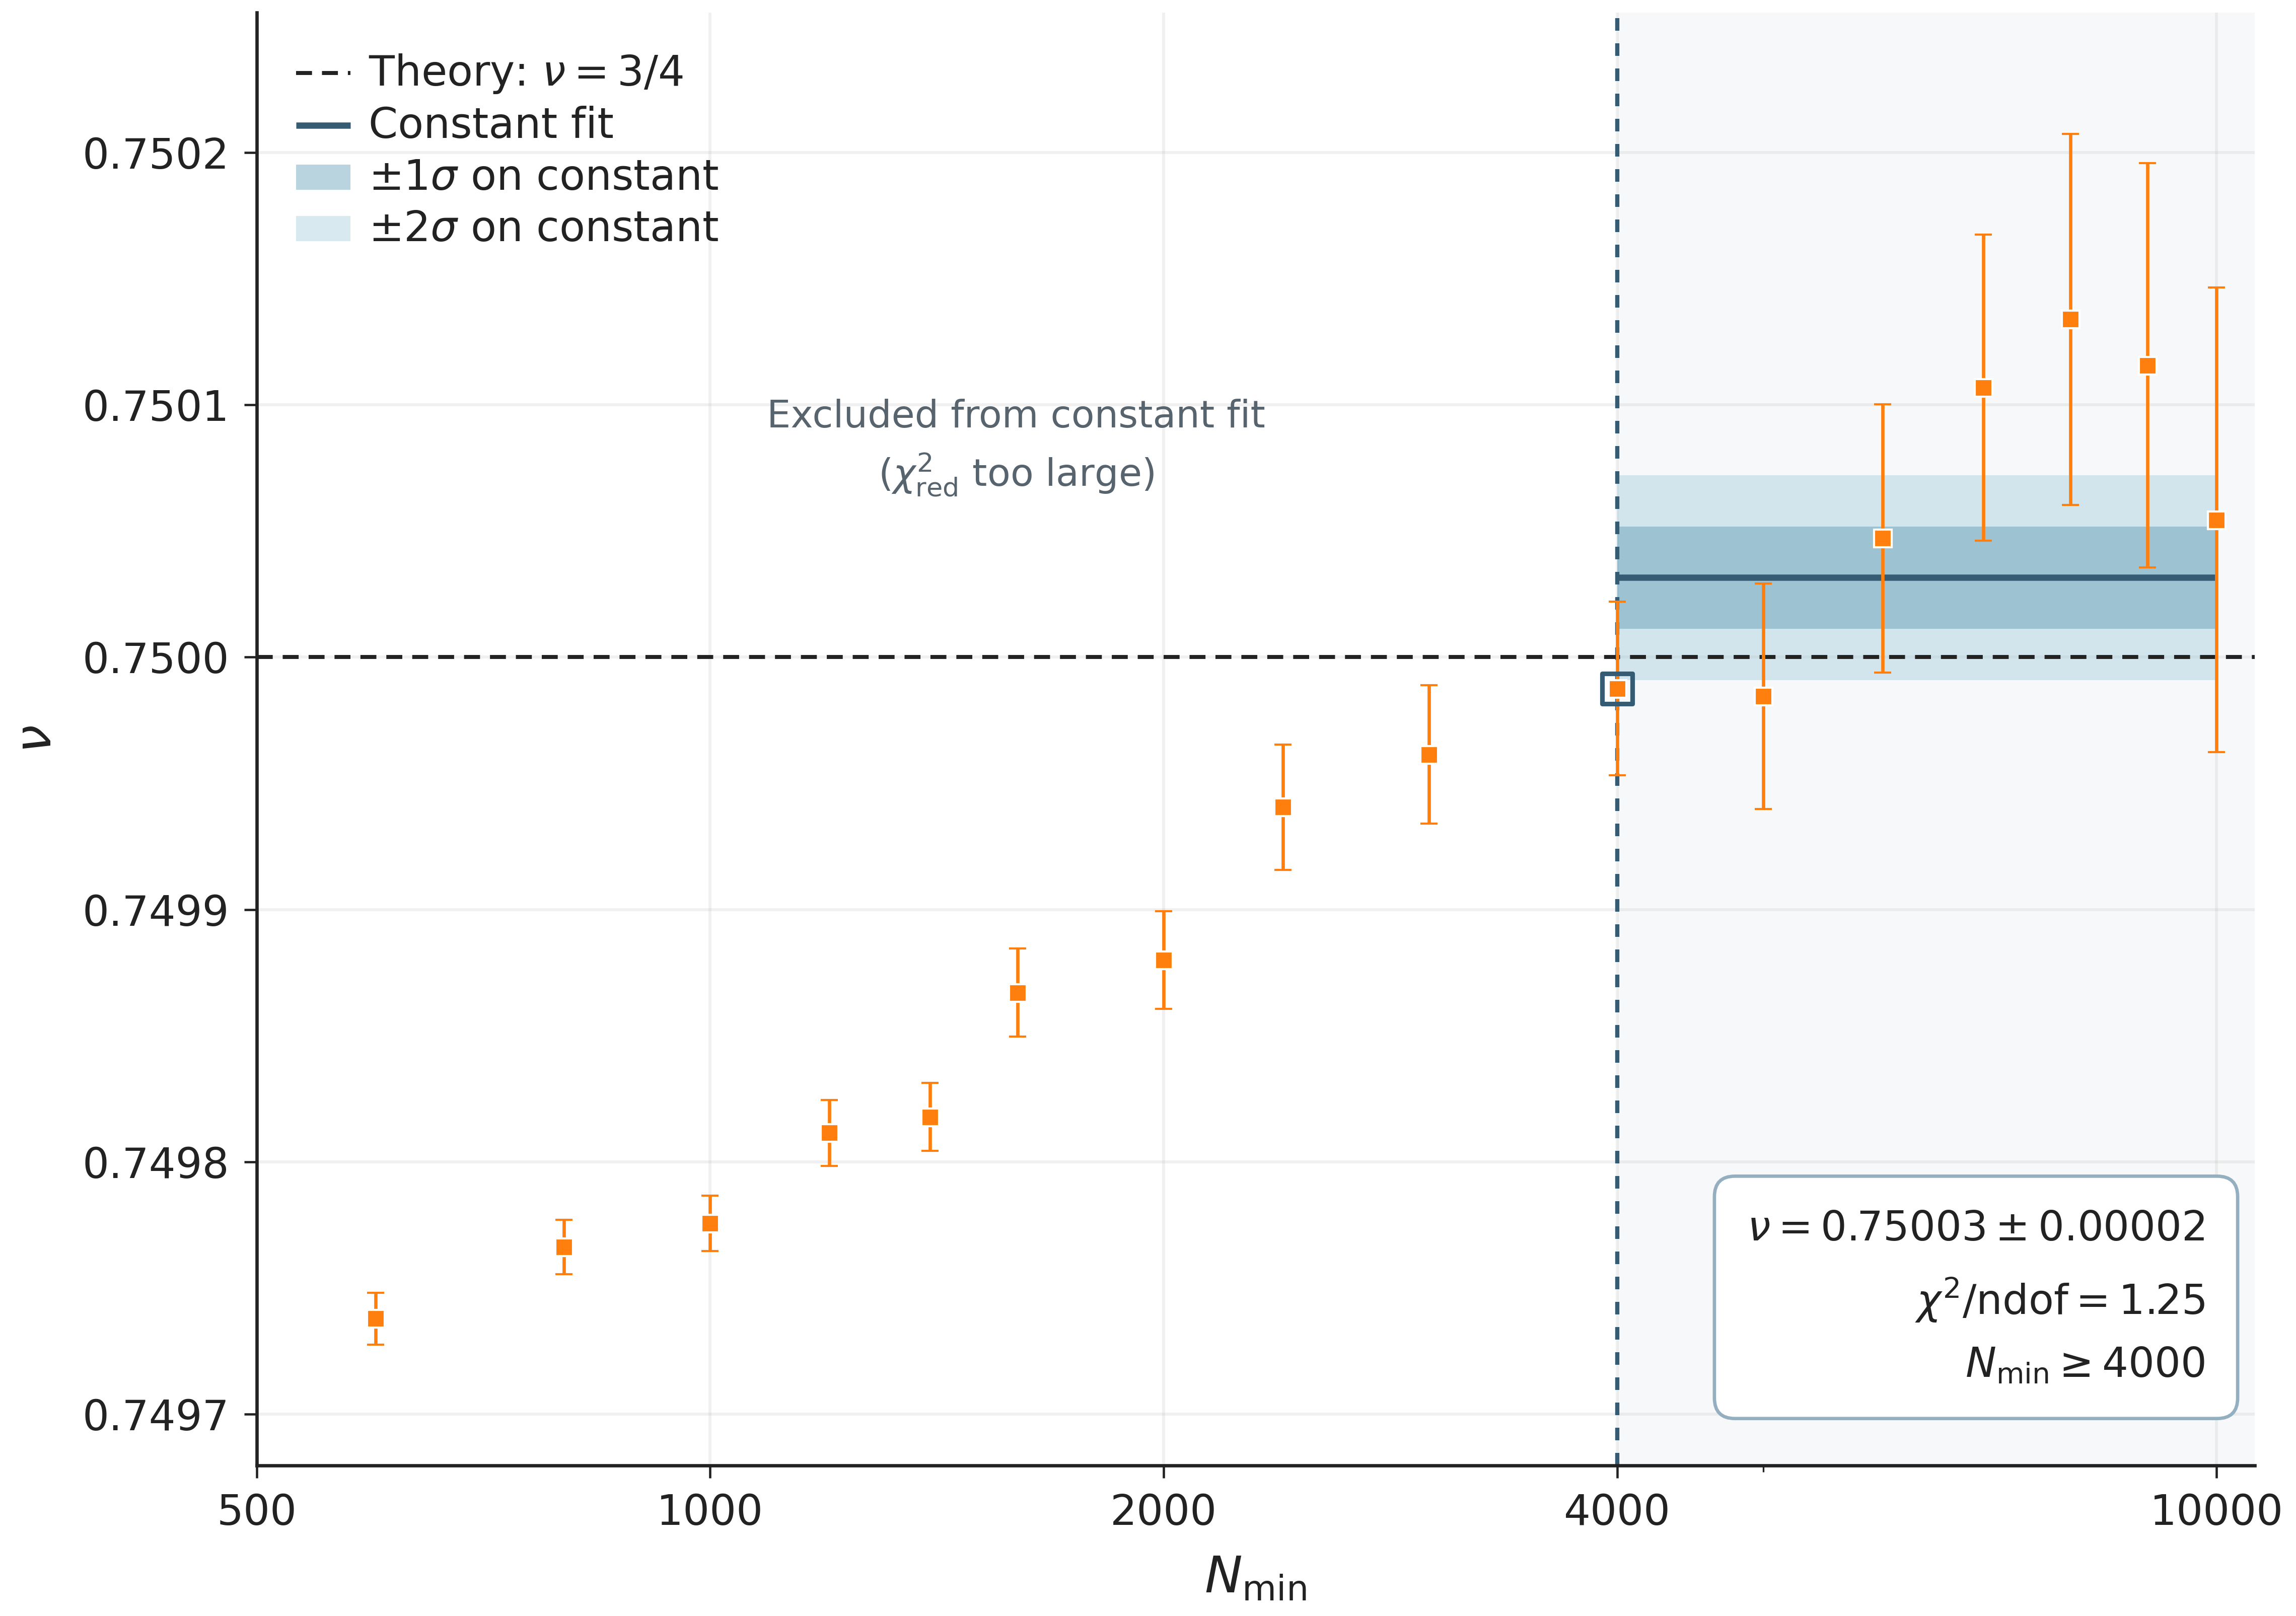
\includegraphics[width=94mm]{09_nu_vs_lmin.png}};
\node[anchor=west,inner sep=0pt,text=ink!75,
font=\fontsize{8.5}{9.5}\selectfont] at (13,86)
{Pivot: power-law fits using $N\geq N_{\min}$};

% Soft panel and small scientific motifs, without a dark banner.
\begin{scope}[shift={(0,-3)}]
\filldraw[fill=ink!2,draw=ink!12,line width=.4pt,rounded corners=1.7mm]
(106,18) rectangle (153,84);
\node[anchor=west,inner sep=0pt,text=ink,
font=\fontsize{10.7}{11.5}\selectfont\bfseries] at (110,24)
{Future directions};
\draw[ink!18,line width=.4pt] (110,29) -- (151,29);
\draw[simple!65!ink,line width=1.1pt,line cap=round] (110,29) -- (119,29);

\node[anchor=north west,inner sep=0pt,text=ink,
font=\fontsize{10}{10.5}\selectfont\bfseries] at (110,35)
{Three dimensions};
\fill[simple!85!ink] (108,36.4) circle (.7mm);
% Wireframe cube evokes the additional spatial dimension.
\begin{scope}[shift={(146,33.5)},draw=ink!45,line width=.45pt]
\draw (0,1.5) rectangle (3.5,5);
\draw (1.5,0) -- (5,0) -- (5,3.5) -- (3.5,5);
\draw (0,1.5) -- (1.5,0);
\draw (3.5,1.5) -- (5,0);
\end{scope}
\node[anchor=north west,text width=41mm,inner sep=0pt,text=ink!85,
font=\fontsize{9}{10.7}\selectfont,align=left] at (110,41)
{SAWs in 3D, closer to\par real polymer geometry.};

\draw[ink!12,line width=.35pt] (110,52) -- (151,52);
\node[anchor=north west,inner sep=0pt,text=ink,
font=\fontsize{10}{10.5}\selectfont\bfseries] at (110,57)
{Interacting SAWs};
\fill[pivot!85!ink] (108,58.4) circle (.7mm);
% Two nonconsecutive sites with a dashed attractive contact.
\begin{scope}[shift={(146,56)},draw=ink!45,line width=.55pt]
\draw (0,0) -- (0,3) -- (4,3) -- (4,0);
\draw[dashed,simple!65!ink] (0,0) -- (4,0);
\foreach \x/\y in {0/0,0/3,4/3,4/0}
  \fill[ink!50] (\x,\y) circle (.38mm);
\end{scope}
\node[anchor=north west,text width=41mm,inner sep=0pt,text=ink!85,
font=\fontsize{9}{10.7}\selectfont,align=left] at (110,63)
{Add attractive contacts\par between nonconsecutive\par neighbours (ISAW).};
\node[anchor=north west,text width=41mm,inner sep=0pt,text=ink!75,
font=\fontsize{8.8}{10.4}\selectfont,align=left] at (110,77)
{Vary solvent quality:\par swollen or compact chains.};
\end{scope}
\end{scope}
\end{tikzpicture}
\end{frame}
\begin{frame}{References}
\small
\begin{thebibliography}{4}
\setlength{\itemsep}{3mm}
\bibitem{gennes} P.-G. de Gennes, \emph{Scaling Concepts in Polymer Physics}, Cornell University Press, Ithaca (1979).
\bibitem{binder} K. Binder and D. W. Heermann, \emph{Monte Carlo Simulation in Statistical Physics: An Introduction}, 4th ed., Springer, Berlin (2002).
\bibitem{pivot} N. Madras and A. D. Sokal, ``The Pivot Algorithm: A Highly Efficient Monte Carlo Method for the Self-Avoiding Walk'', \emph{Journal of Statistical Physics} \textbf{50}, 109--186 (1988).
\bibitem{scaling} S. Caracciolo, A. J. Guttmann, I. Jensen, A. Pelissetto, A. N. Rogers and A. D. Sokal, ``Correction-to-Scaling Exponents for Two-Dimensional Self-Avoiding Walks'', \emph{Journal of Statistical Physics} \textbf{120}, 1037--1100 (2005).
\end{thebibliography}
\end{frame}

\begin{frame}[plain,noframenumbering]
\centering
{\Huge Backup}
\end{frame}

% Backup derivation: algebra is conditional on the stated physical approximations.
\begin{frame}{Flory free energy: entropy and excluded volume}
\begin{tikzpicture}[remember picture,overlay]
\begin{scope}[shift={(current page.north west)},x=1mm,y=-1mm]
\node[anchor=north west,text width=145mm,inner sep=0pt,
font=\fontsize{9}{10.5}\selectfont] at (7,12)
{$N$ bonds of length $a$, spatial extent $R=|\mathbf R|$, and $1<d<4$.\par
Long-chain, good-solvent regime: $N+1\simeq N\gg1$ monomers and $v>0$.};

\node[anchor=west,inner sep=0pt,text=simple,
font=\fontsize{10.5}{11.5}\selectfont\bfseries] at (10,26) {Gaussian elastic cost};
\node[anchor=west,inner sep=0pt,
font=\fontsize{9.8}{11}\selectfont] at (10,36)
{$\displaystyle P_0(\mathbf R)\simeq
 \left(\frac{d}{2\pi Na^2}\right)^{d/2}
 \exp\!\left[-\frac{dR^2}{2Na^2}\right]$};
\node[anchor=west,inner sep=0pt,
font=\fontsize{10.2}{11.5}\selectfont] at (10,49)
{$\displaystyle \frac{F_{\rm el}}{k_{\rm B}T}
=-\ln P_0+\mathrm{const}
=C_{\rm el}\frac{R^2}{Na^2}$};
\node[anchor=north west,text width=66mm,inner sep=0pt,text=ink!75,
font=\fontsize{8.5}{9.5}\selectfont] at (10,55)
{Ideal-chain reference: stretching reduces entropy.};

\draw[ink!15,line width=.4pt] (79,25) -- (79,58);
\node[anchor=west,inner sep=0pt,text=pivot,
font=\fontsize{10.5}{11.5}\selectfont\bfseries] at (84,26) {Pair excluded volume};
\node[anchor=west,inner sep=0pt,
font=\fontsize{10.2}{11.5}\selectfont] at (84,35)
{$\displaystyle V=\kappa_d R^d,\qquad \rho\simeq\frac{N}{V}$};
\node[anchor=west,inner sep=0pt,
font=\fontsize{10.2}{11.5}\selectfont] at (84,45)
{$\displaystyle \frac{F_{\rm rep}}{k_{\rm B}T}
\simeq\frac{v}{2}\int \rho(\mathbf r)^2\,\mathrm d^d r
=\frac{vN^2}{2V}$};
\node[anchor=west,inner sep=0pt,
font=\fontsize{10.2}{11.5}\selectfont] at (84,55)
{$\displaystyle \frac{F_{\rm rep}}{k_{\rm B}T}
=C_{\rm rep}\frac{vN^2}{R^d}$};

\node[anchor=north west,text width=145mm,inner sep=0pt,text=ink!80,
font=\fontsize{8.2}{9.5}\selectfont] at (7,61)
{\textbf{Approximations:} Gaussian elasticity, uniform density and local pair repulsion.\par
Spatial correlations and higher density terms are omitted. $v$ has units of length$^d$.};

\fill[simple!7,rounded corners=1mm] (7,69) rectangle (153,79);
\node[font=\fontsize{12}{13}\selectfont] at (80,74)
{$\displaystyle \Phi(R)\equiv\frac{F_{\rm F}(R)}{k_{\rm B}T}
={\color{simple}C_{\rm el}\frac{R^2}{Na^2}}
+{\color{pivot}C_{\rm rep}\frac{vN^2}{R^d}}$};
\node[anchor=west,inner sep=0pt,text=ink!75,
font=\fontsize{7.5}{8.5}\selectfont] at (9,82)
{$C_{\rm el}=d/2,\quad C_{\rm rep}=1/(2\kappa_d)>0$:
prefactors do not depend on $N$ or $R$.};
\node[anchor=west,inner sep=0pt,text=ink!65,
font=\fontsize{6.5}{7.5}\selectfont] at (7,87)
{de Gennes (1979); \href{https://ocw.mit.edu/courses/18-366-random-walks-and-diffusion-fall-2006/f55c3437987782c16c8910266cdc6ddc_lec19.pdf}{Bazant, Polymer Models, Sec.~3.2}.};
\end{scope}
\end{tikzpicture}
\end{frame}

\begin{frame}{From the free-energy minimum to the power law}
\begin{tikzpicture}[remember picture,overlay]
\begin{scope}[shift={(current page.north west)},x=1mm,y=-1mm]
\node[anchor=west,inner sep=0pt,text=simple,
font=\fontsize{10}{11}\selectfont\bfseries] at (8,14)
{Minimum of the Flory free energy};
\node[anchor=west,inner sep=0pt,
font=\fontsize{10.5}{11.5}\selectfont] at (9,24)
{$\displaystyle \Phi'(R_*)=
\frac{2C_{\rm el}R_*}{Na^2}
-\frac{dC_{\rm rep}vN^2}{R_*^{d+1}}=0
\quad\Longrightarrow\quad
R_*^{d+2}=\frac{dC_{\rm rep}}{2C_{\rm el}}\,va^2N^3$};
\node[anchor=west,inner sep=0pt,
font=\fontsize{10.5}{11.5}\selectfont] at (9,36)
{$\displaystyle v\sim a^d
\quad\Longrightarrow\quad
R_*\sim aN^{\nu_{\rm F}},\qquad
\nu_{\rm F}=\frac{3}{d+2}$};
\node[anchor=west,inner sep=0pt,
font=\fontsize{9.5}{10.5}\selectfont] at (9,46)
{$\displaystyle \Phi''(R)=
\frac{2C_{\rm el}}{Na^2}
+\frac{d(d+1)C_{\rm rep}vN^2}{R^{d+2}}>0
\quad(R>0):\ \text{unique minimum}$};

\node[anchor=west,inner sep=0pt,text=pivot,
font=\fontsize{10}{11}\selectfont\bfseries] at (8,54)
{Second moment: assume one characteristic length};
\node[anchor=west,inner sep=0pt,
font=\fontsize{10.2}{11.5}\selectfont] at (9,62)
{$\displaystyle P_N(\mathbf R)\simeq\ell_N^{-d}p(\mathbf R/\ell_N),
\quad \ell_N=aBN^\nu,\quad
\int p(\mathbf x)\,\mathrm d^d x=1$};
\node[anchor=west,inner sep=0pt,
font=\fontsize{10.2}{11.5}\selectfont] at (9,71)
{$\displaystyle
\langle R_e^2\rangle=\int R^2P_N(\mathbf R)\,\mathrm d^d R
\simeq\ell_N^2\underbrace{\int|\mathbf x|^2p(\mathbf x)\,\mathrm d^d x}_{C_2<\infty}
=A N^{2\nu}$};
\fill[ink,rounded corners=1mm] (7,79) rectangle (153,84.5);
\node[anchor=west,inner sep=0pt,text=white,
font=\fontsize{8.5}{9.5}\selectfont] at (10,81.75)
{$A=a^2B^2C_2$};
\node[text=white,font=\fontsize{11.5}{12.5}\selectfont] at (99,81.75)
{$d=2:\quad \nu_{\rm F}=3/4
\quad\Longrightarrow\quad \langle R_e^2\rangle\sim A N^{3/2}$};
\node[anchor=west,inner sep=0pt,text=ink!75,
font=\fontsize{7}{8}\selectfont] at (7,86)
{Conditional derivation under Flory/scaling assumptions, not a rigorous proof for lattice SAWs.};
\node[anchor=west,inner sep=0pt,text=ink!65,
font=\fontsize{6.2}{7}\selectfont] at (7,88.5)
{\href{https://arxiv.org/pdf/cond-mat/0409355}{Caracciolo et al. (2005), Sec.~2};
\href{https://www.ihes.fr/~duminil/publi/saw_lecture_notes.pdf}{Bauerschmidt et al. (2012), Sec.~1.6}: planar prediction $\nu=3/4$.};
\end{scope}
\end{tikzpicture}
\end{frame}

\begin{frame}{Finite-size corrections: a broader fit range}
\begin{tikzpicture}[remember picture,overlay]
\begin{scope}[shift={(current page.north west)},x=1mm,y=-1mm]
\node[anchor=west,inner sep=0pt,font=\fontsize{12}{14}\selectfont] at (9,17)
{$\displaystyle \langle R_e^2\rangle=A N^{2\nu}\left(1+\frac{b}{N}+\frac{c}{N^{3/2}}\right)$};
\node[anchor=north west,inner sep=0pt] at (5,23)
{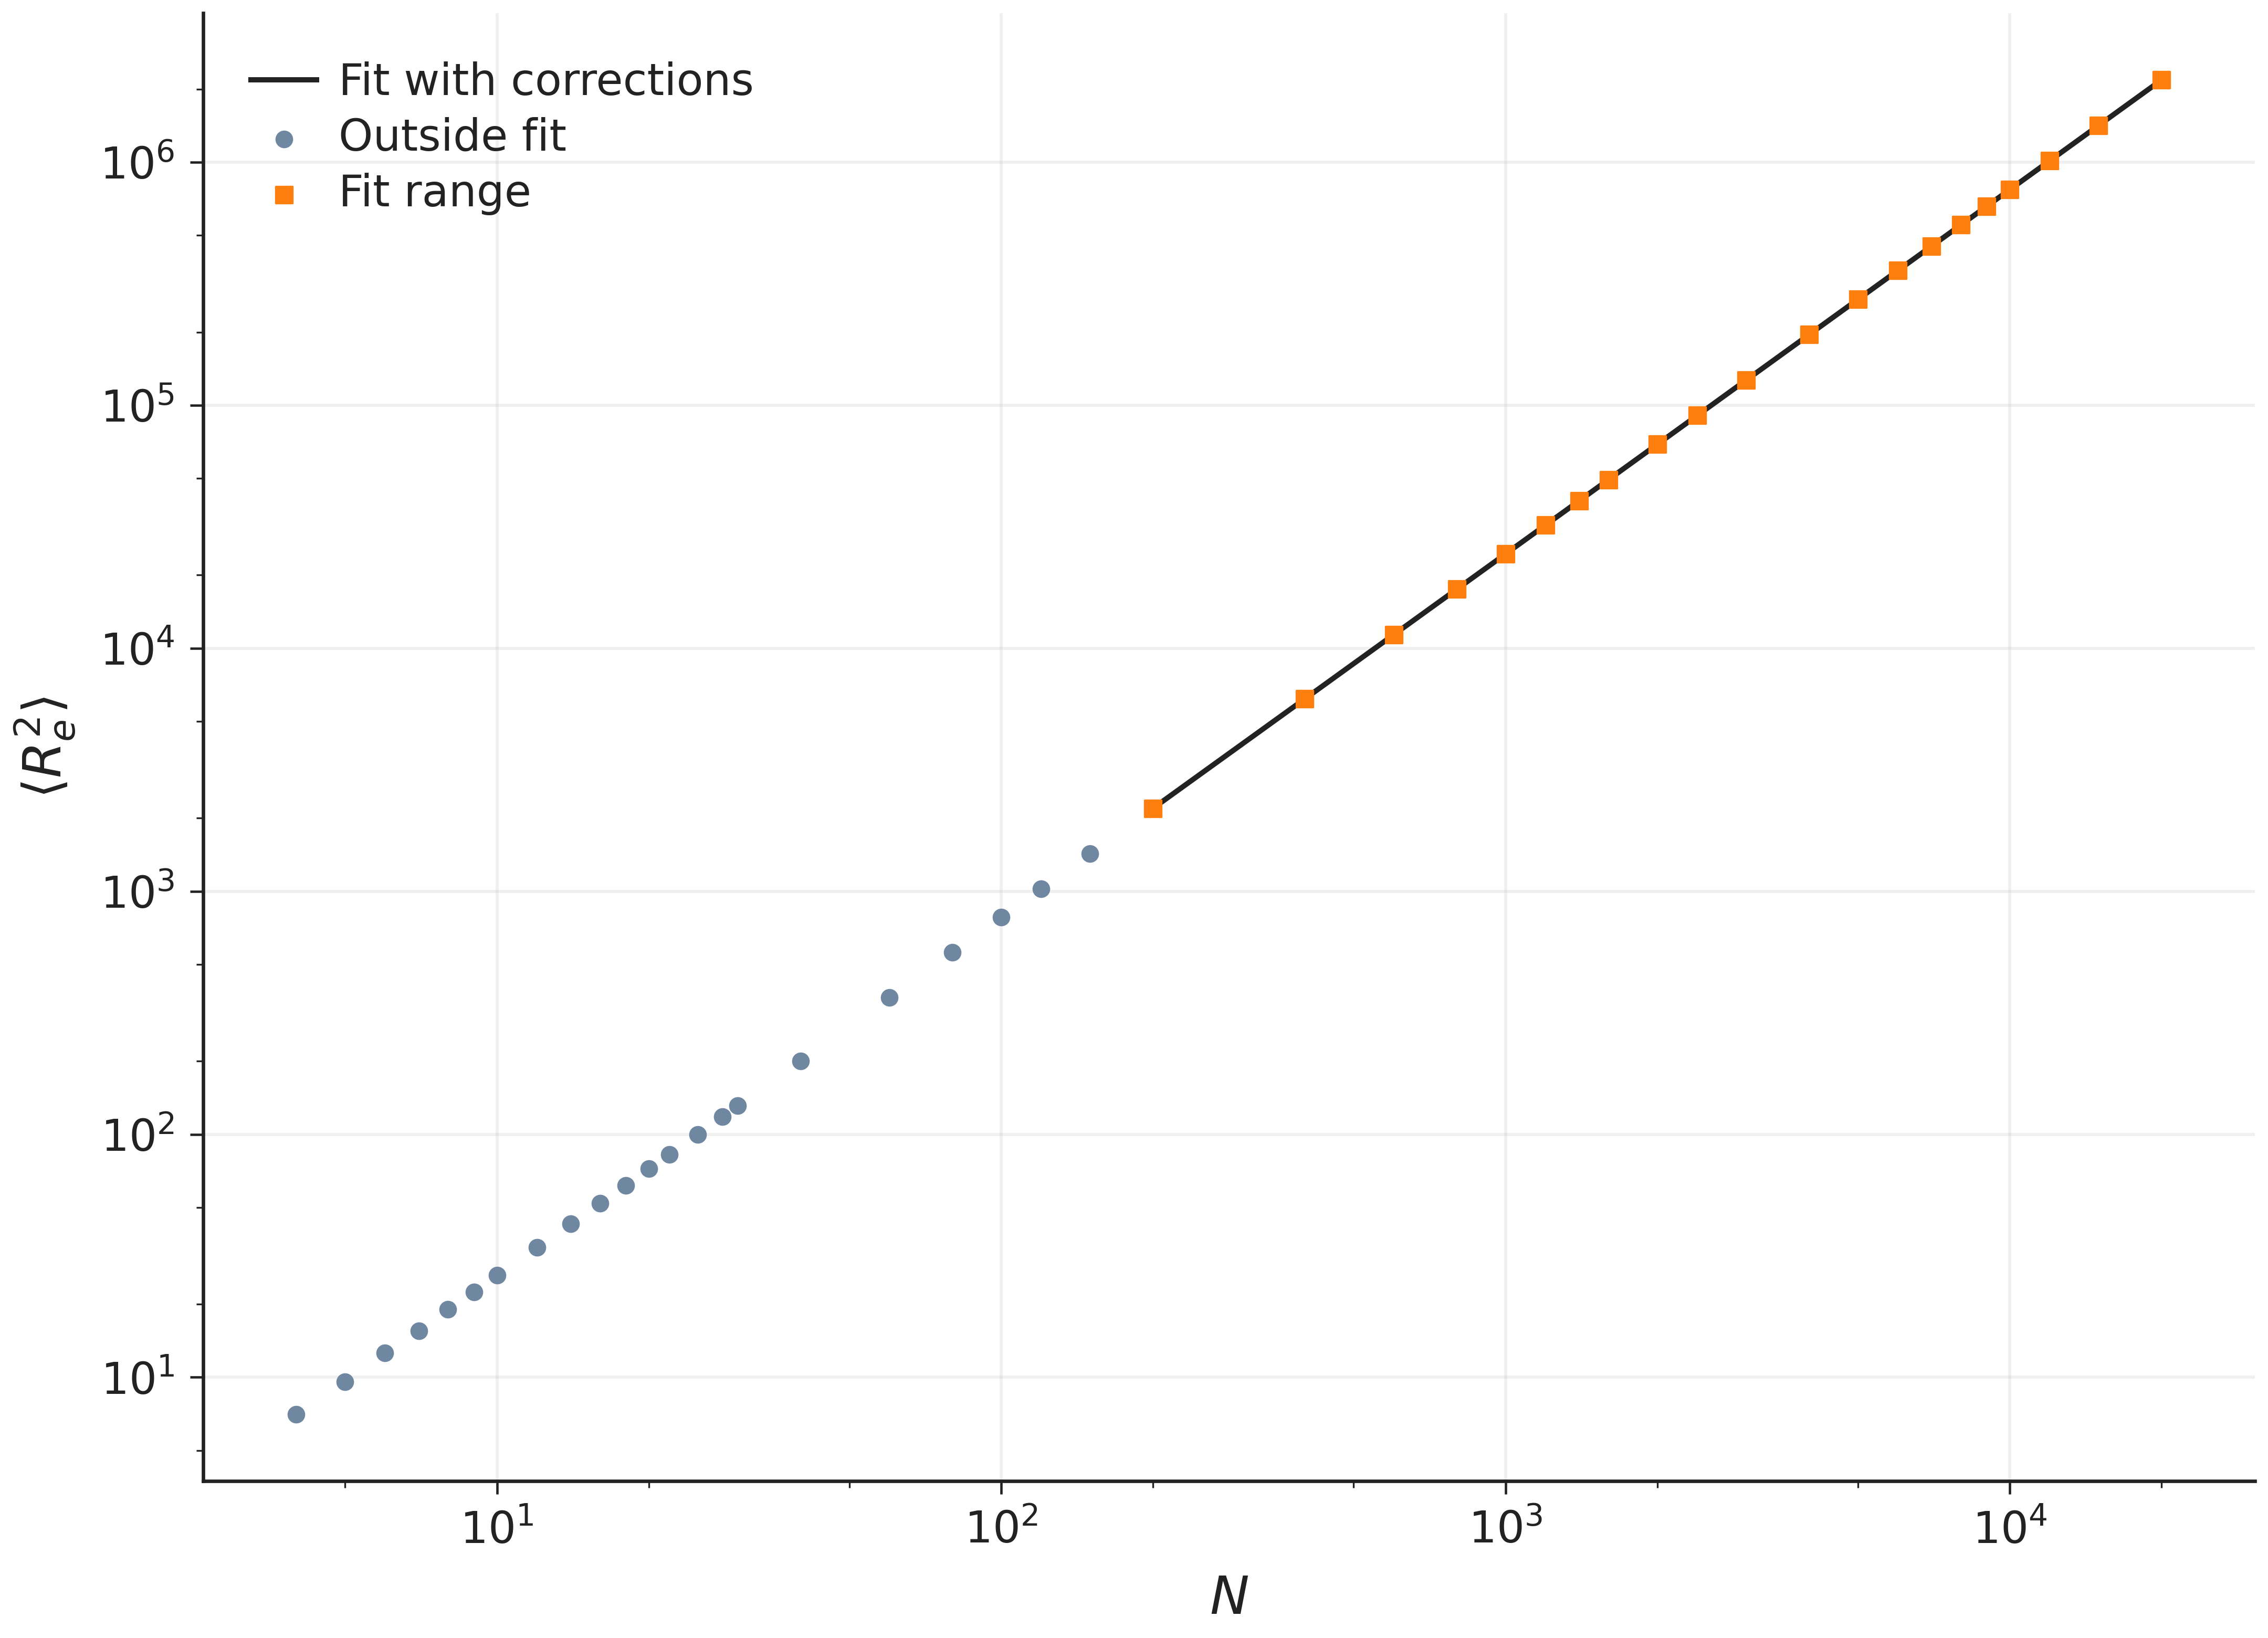
\includegraphics[width=84mm]{backup_pivot_corrections.png}};
\begin{scope}[shift={(0,-3)}]
\filldraw[fill=ink!2,draw=ink!12,line width=.4pt,rounded corners=1.5mm]
(98,26) rectangle (153,81);
\draw[pivot,line width=1.1pt,line cap=round] (102,28.5) -- (117,28.5);
\node[anchor=west,inner sep=0pt,text=pivot,font=\fontsize{10.5}{12}\selectfont\bfseries] at (102,32)
{Pivot fit results};
\node[anchor=west,inner sep=0pt,font=\fontsize{10}{11}\selectfont] at (102,39)
{$200\leq N\leq20000$};
\fill[pivot!7,rounded corners=.9mm] (101,43) rectangle (150,52);
\node[anchor=west,inner sep=0pt,font=\fontsize{11}{12}\selectfont] at (102,48)
{$\nu=\correctedNu$};
\node[anchor=west,inner sep=0pt,font=\fontsize{9}{10}\selectfont] at (102,55)
{$\chi^2/\mathrm{ndof}=\correctedReducedChi\quad(\mathrm{ndof}=\correctedDof)$};
\draw[ink!12,line width=.4pt] (102,59) -- (149,59);
\node[anchor=west,inner sep=0pt,font=\fontsize{9}{10}\selectfont] at (102,64)
{$A=\correctedA$};
\node[anchor=west,inner sep=0pt,font=\fontsize{9}{10}\selectfont] at (102,70)
{$b=\correctedB$};
\node[anchor=west,inner sep=0pt,font=\fontsize{9}{10}\selectfont] at (102,76)
{$c=\correctedC$};
\end{scope}
\node[anchor=west,inner sep=0pt,text=ink!75,font=\fontsize{7.8}{9}\selectfont] at (9,86)
{Four free parameters; fixed correction powers. Errors: one standard deviation.};
\end{scope}
\end{tikzpicture}
\end{frame}

\begin{frame}{Future models: three dimensions and attractive contacts}
\begin{tikzpicture}[remember picture,overlay]
\begin{scope}[shift={(current page.north west)},x=1mm,y=-1mm]
\node[anchor=west,inner sep=0pt,text=simple,
font=\fontsize{11}{12}\selectfont\bfseries] at (9,16)
{Three-dimensional SAWs};
\node[anchor=center,inner sep=0pt] at (39,37) {
\begin{tikzpicture}[x={(.65cm,-.15cm)},y={(.32cm,.35cm)},z={(0cm,.65cm)},scale=.78,>=stealth]
\foreach \z in {0,1,2,3}{
  \foreach \y in {0,1,2}{\draw[ink!11,thin] (0,\y,\z)--(3,\y,\z);}
  \foreach \x in {0,1,2,3}{\draw[ink!11,thin] (\x,0,\z)--(\x,2,\z);}
}
\foreach \x in {0,1,2,3}{\foreach \y in {0,1,2}{\draw[ink!11,thin] (\x,\y,0)--(\x,\y,3);}}
\draw[simple,line width=1.4pt] (0,0,0)--(1,0,0)--(1,1,0)--(1,1,1)--(2,1,1)--(2,2,1)--(2,2,2)--(1,2,2)--(0,2,2)--(0,1,2)--(0,1,3)--(1,1,3)--(2,1,3)--(2,0,3)--(3,0,3)--(3,0,2)--(3,1,2)--(3,1,1)--(3,2,1)--(3,2,0)--(2,2,0);
\fill[simple] (0,0,0) circle(.055cm);
\fill[simple] (1,0,0) circle(.055cm);
\fill[simple] (1,1,0) circle(.055cm);
\fill[simple] (1,1,1) circle(.055cm);
\fill[simple] (2,1,1) circle(.055cm);
\fill[simple] (2,2,1) circle(.055cm);
\fill[simple] (2,2,2) circle(.055cm);
\fill[simple] (1,2,2) circle(.055cm);
\fill[simple] (0,2,2) circle(.055cm);
\fill[simple] (0,1,2) circle(.055cm);
\fill[simple] (0,1,3) circle(.055cm);
\fill[simple] (1,1,3) circle(.055cm);
\fill[simple] (2,1,3) circle(.055cm);
\fill[simple] (2,0,3) circle(.055cm);
\fill[simple] (3,0,3) circle(.055cm);
\fill[simple] (3,0,2) circle(.055cm);
\fill[simple] (3,1,2) circle(.055cm);
\fill[simple] (3,1,1) circle(.055cm);
\fill[simple] (3,2,1) circle(.055cm);
\fill[simple] (3,2,0) circle(.055cm);
\fill[simple] (2,2,0) circle(.055cm);
\fill[ink] (0,0,0) circle(.09cm);
\fill[pivot] (2,2,0) circle(.09cm);
\draw[->,ink!60,line width=.7pt] (-1.1,-.9,0)--(-.3,-.9,0) node[below,font=\fontsize{7}{8}\selectfont] {$x$};
\draw[->,ink!60,line width=.7pt] (-1.1,-.9,0)--(-1.1,-.1,0) node[right,font=\fontsize{7}{8}\selectfont] {$y$};
\draw[->,ink!60,line width=.7pt] (-1.1,-.9,0)--(-1.1,-.9,.8) node[left,font=\fontsize{7}{8}\selectfont] {$z$};
\end{tikzpicture}};
\node[anchor=north west,text width=62mm,inner sep=0pt,
font=\fontsize{9}{10.6}\selectfont] at (9,55)
{Cubic lattice: steps along $\pm x,\pm y,\pm z$.\par\vspace{1.2mm}
Use cubic-lattice symmetries for Pivot moves.\par\vspace{1.2mm}
Numerical reference: $\nu_{\rm 3D}\simeq0.588$.\par
Flory estimates $3/5$, illustrating its limits.};

\draw[ink!15,line width=.4pt] (76,15) -- (76,82);
\node[anchor=west,inner sep=0pt,text=pivot,
font=\fontsize{11}{12}\selectfont\bfseries] at (82,16)
{Interacting SAWs (ISAW)};
\node[anchor=center,inner sep=0pt] at (99,33) {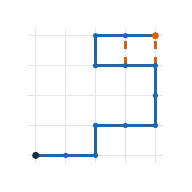
\begin{tikzpicture}[x=1cm,y=1cm,scale=.38]
\draw[step=1,ink!12,thin] (-.25,-.25) grid (4.25,4.25);
\draw[pivot,dashed,line width=.85pt] (4,3)--(4,4) (3,3)--(3,4);
\draw[simple,line width=1.25pt] (0,0)--(1,0)--(2,0)--(2,1)--(3,1)--(4,1)--(4,2)--(4,3)--(3,3)--(2,3)--(2,4)--(3,4)--(4,4);
\fill[simple] (0,0) circle(.09);
\fill[simple] (1,0) circle(.09);
\fill[simple] (2,0) circle(.09);
\fill[simple] (2,1) circle(.09);
\fill[simple] (3,1) circle(.09);
\fill[simple] (4,1) circle(.09);
\fill[simple] (4,2) circle(.09);
\fill[simple] (4,3) circle(.09);
\fill[simple] (3,3) circle(.09);
\fill[simple] (2,3) circle(.09);
\fill[simple] (2,4) circle(.09);
\fill[simple] (3,4) circle(.09);
\fill[simple] (4,4) circle(.09);
\fill[ink] (0,0) circle(.12);
\fill[pivot] (4,4) circle(.12);
\end{tikzpicture}};
\node[anchor=center,inner sep=0pt] at (135,33) {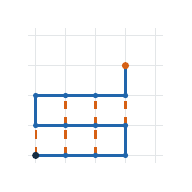
\begin{tikzpicture}[x=1cm,y=1cm,scale=.38]
\draw[step=1,ink!12,thin] (-.25,-.25) grid (4.25,4.25);
\draw[pivot,dashed,line width=.85pt] (0,0)--(0,1) (1,0)--(1,1) (2,0)--(2,1) (3,1)--(3,2) (2,1)--(2,2) (1,1)--(1,2);
\draw[simple,line width=1.25pt] (0,0)--(1,0)--(2,0)--(3,0)--(3,1)--(2,1)--(1,1)--(0,1)--(0,2)--(1,2)--(2,2)--(3,2)--(3,3);
\fill[simple] (0,0) circle(.09);
\fill[simple] (1,0) circle(.09);
\fill[simple] (2,0) circle(.09);
\fill[simple] (3,0) circle(.09);
\fill[simple] (3,1) circle(.09);
\fill[simple] (2,1) circle(.09);
\fill[simple] (1,1) circle(.09);
\fill[simple] (0,1) circle(.09);
\fill[simple] (0,2) circle(.09);
\fill[simple] (1,2) circle(.09);
\fill[simple] (2,2) circle(.09);
\fill[simple] (3,2) circle(.09);
\fill[simple] (3,3) circle(.09);
\fill[ink] (0,0) circle(.12);
\fill[pivot] (3,3) circle(.12);
\end{tikzpicture}};
\node[font=\fontsize{8.2}{9.2}\selectfont,text=simple] at (99,44)
{Swollen: $m=2$};
\node[font=\fontsize{8.2}{9.2}\selectfont,text=pivot] at (135,44)
{Compact: $m=6$};
\node[anchor=west,inner sep=0pt,text=ink!70,
font=\fontsize{7.6}{8.6}\selectfont] at (83,50)
{Same $N=12$; dashed lines mark nonbonded contacts.};
\node[anchor=west,inner sep=0pt,
font=\fontsize{10.7}{12}\selectfont] at (83,59)
{$E=-\varepsilon m,\quad\varepsilon>0,\qquad
\pi(\omega)\propto e^{\beta\varepsilon m(\omega)}$};
\node[anchor=north west,text width=68mm,inner sep=0pt,
font=\fontsize{8.3}{9.7}\selectfont] at (83,64)
{$m$: nonbonded nearest-neighbour contact pairs.\par
Larger $\beta\varepsilon$ favours compact conformations.};
\node[anchor=west,inner sep=0pt,
font=\fontsize{9.6}{10.6}\selectfont] at (83,75)
{$P_{\rm acc}=\min(1,e^{-\beta\Delta E}),\quad \beta=(k_{\rm B}T)^{-1}$};
\node[anchor=west,inner sep=0pt,text=ink!70,
font=\fontsize{7.4}{8.4}\selectfont] at (83,81)
{Symmetric valid proposals; reject all site overlaps.};
\node[anchor=west,inner sep=0pt,text=ink!65,
font=\fontsize{6.3}{7.3}\selectfont] at (7,87)
{Schematic configurations, not simulation results.
\href{https://arxiv.org/abs/1002.0494}{Clisby, PRL 104, 055702 (2010)};
\href{https://www.staff.uni-mainz.de/hsu/mypaper/JPA02-polymer.pdf}{Hsu and Grassberger, J.~Phys.~A 35, L759 (2002)}.};
\end{scope}
\end{tikzpicture}
\end{frame}

\end{document}
